\section{Методика использования программного средства}
\label{sec:manual}

В данном разделе приведены основные сведения по работе с программным средством.

Приложение данного дипломного проекта (а точнее, его клиентская\linebreak часть) не требует установки и настройки на конечных устройствах пользователя, поскольку представляет собой веб-приложение. Как и было заявлено в требованиях, для корректной работы программного средства необходим один из следующих браузеров с соответствующей минимальной версией:
\begin{itemize}
	\item Google Chrome 49;
	\item Vivaldi 1.0;
	\item Opera 34;
	\item Mozilla Firefox 43;
	\item Apple Safari 9.0;
	\item Microsoft Edge 20.
\end{itemize}

Далее рассмотрены основные функции, предоставляемые приложением пользователям.

При открытии главной страницы приложения отображается экран расписания (рисунок~\ref{fig:manual:agenda_screen}). Для того, чтобы отобразить расписание уже пройденных занятий, следует нажать кнопку <<Предыдущая неделя>>. Для выбора даты для отображения расписания следует нажать кнопку с пиктограммой календаря.

\begin{figure}[ht]
\centering
	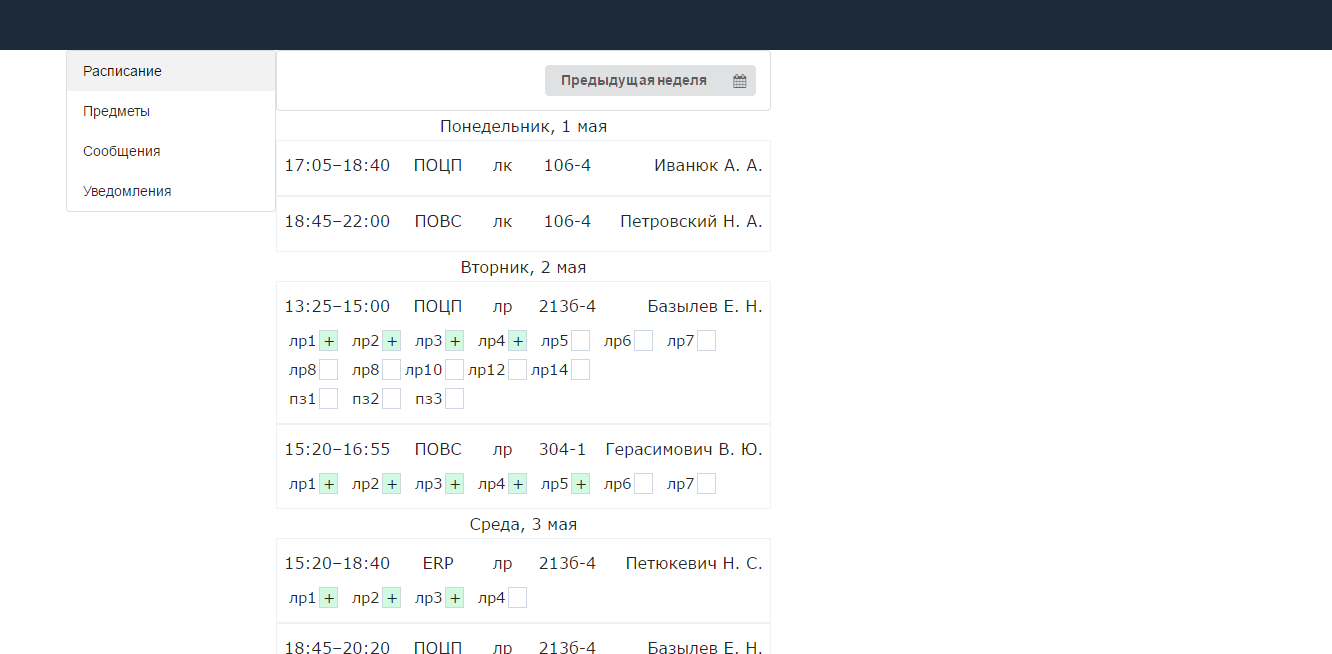
\includegraphics[scale=0.36]{agenda_screen.png}
	\caption{Экран расписания}
	\label{fig:manual:agenda_screen}
\end{figure}

Далее, при нажатии на строку расписания в правой части приложения отображается страница с детальной информацией о предмете (рисунок~\ref{fig:manual:discipline_page}). При наведении на его аббревиатуру отображается его полное название, а при наведении на фамилию преподавателя -- его полное имя. На данной странице можно просмотреть материалы по этому предмету, которые добавил преподаватель, список индивидуальных заданий. Кроме того, на данной странице есть возможность сразу написать некоторое сообщение преподавателю.

\begin{figure}[ht]
\centering
	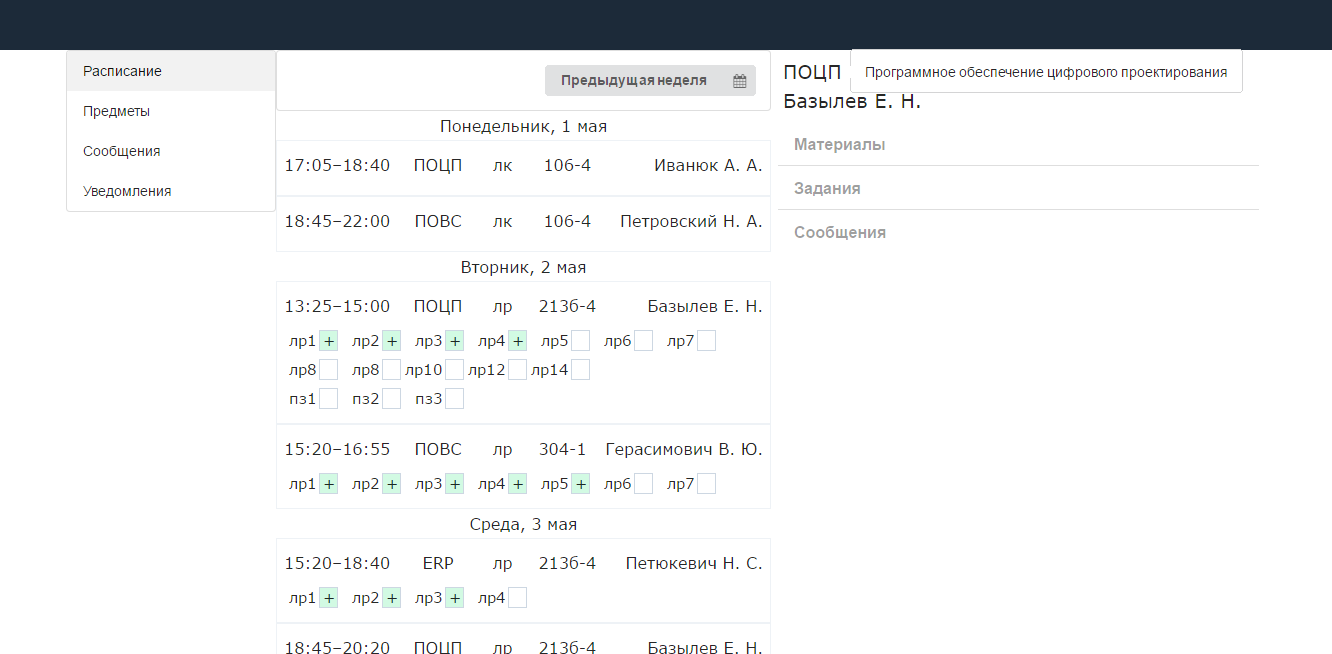
\includegraphics[scale=0.36]{discipline_page.png}
	\caption{Экран расписания с открытой страницей предмета}
	\label{fig:manual:discipline_page}
\end{figure}

Для открытия экрана со списком предметов (рисунок~\ref{fig:manual:disciplines_screen}) следует нажать кнопку <<Предметы>> в главном меню, расположенном слева. На данной странице также есть возможность просмотра детальной информации о предмете, для этого необходимо выбрать один из списка.

\begin{figure}[ht!]
\centering
	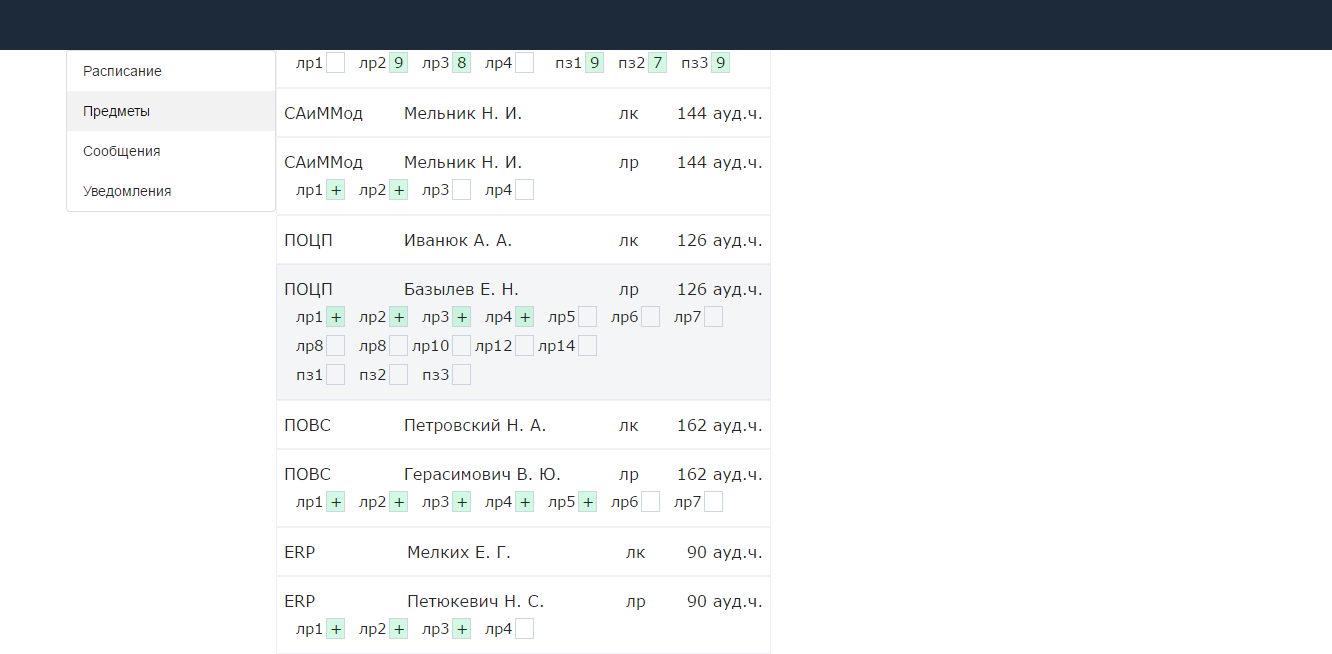
\includegraphics[scale=0.36]{disciplines_screen.png}
	\caption{Экран предметов}
	\label{fig:manual:disciplines_screen}
\end{figure}

Кроме того, на данном экране, а также на ранее рассмотренном экране есть возможность выбора и просмотра детальной информации об индивидуальных заданиях. Для этого нужно нажать соответствующую кнопку в строке предмета. На странице задания (рисунок~\ref{fig:manual:task_page}) можно просмотреть его условие, а также отправить результаты выполнения. Кроме того, на данной странице также есть возможность отправки сообщений преподавателю.

\begin{figure}[ht!]
\centering
	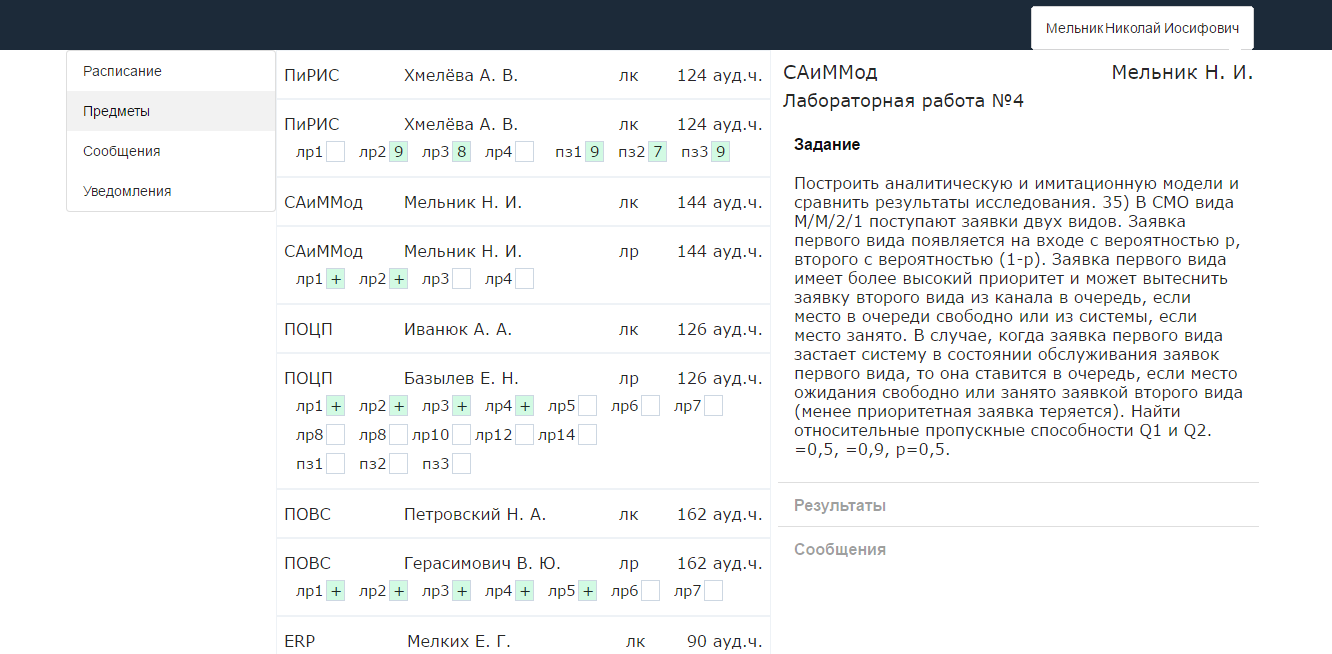
\includegraphics[scale=0.36]{task_page.png}
	\caption{Экран предметов с открытой страницей задания}
	\label{fig:manual:task_page}
\end{figure}

Таким образом, в данном разделе приведены примеры использования некоторых их основных возможностей разработанного программного средства. Следование им должно значительно упростить выполнение некоторых рутинных задач студентов и преподавателей.
